The first model I took in consideration is a lightly modified version of the one presented in section \ref{chapter:mat_formulation}. This formula still doesn't adopt the Sub-tour Elimination Constraint (SEC) since it is intended to be used jointly with other SECs and with other methods such as matheuristics.\\
This configuration gives an undirected complete graph $G=(V,E)$. The formulation used in the code is the following:
%\begin{comment}
	\begin{equation}
	\label{eqn:cost-2}
	min\sum_{(i,j)\in A}c_{ij}x_{ij}
	\stepcounter{equation}\tag{{\theequation}a}
	\end{equation}
	
	\begin{equation}
	\label{eqn:in-2}
	\sum_{(i,j)\delta^-(j)}x_{ij}=1, \quad j\in V
	\tag{{\theequation}b}
	\end{equation}
	
	\begin{equation}
	\label{eqn:out-2}
	\sum_{(i,j)\delta^+(j)}x_{ij}=1, \quad i\in V
	\tag{{\theequation}c}
	\end{equation}
	
	\begin{equation}
	x_{ij}\ge 0 \; \text{intero} , \quad (i, j) \in A
	\tag{{\theequation}e}
	\end{equation}
%\end{comment}


It is the same model used in section \ref{chapter:mat_formulation} but in this case \ref{eqn:ragg} is not included.\\
In this implementation, the graph is symmetric. The arcs $(i, j)$ and $(j, i)$ have the same weight and then thus are represented with the same edge. In this way, the total number of variables are reduced too, considering the starting point not of $n^2$, but only $\frac{n(n-1)}{2}$.\\
The result using this model can be seen in figure \ref{fig:basic_model}.

\begin{figure}[h]
	\centering
	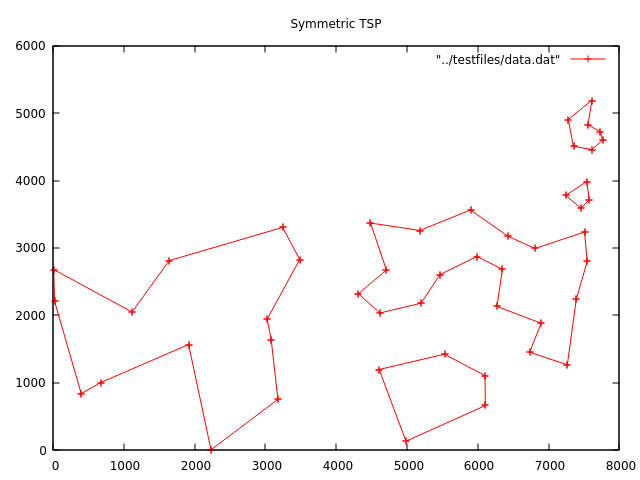
\includegraphics[width=0.6\textwidth]{images/symmetric_with_tours.png}
	\caption{The image represent att48.tsp solved with the problem formulation showed in section \ref{chapter:basic_model}}
	\label{fig:basic_model}
\end{figure}

Since sub-tours are present, this solution cannot be accepted. In the next sections SEC constraints will be added to the formula for avoiding this problem.